\section{Frequency Filtration}
\label{sec:filtering}
The previous section provides motivation for finding ways to reduce the
number of points in the signal and also the number of oscillators that the
signal contains. This has led to work on a procedure for generating
frequency-filtered ``sub-FIDs'' from the original data. A detailed description
of the filtering procedure is presented in this section.

\subsection{The \acl{VE}}
\label{subsec:ve}
In brief, the filtering procedure  consists taking the \ac{FT} of the \ac{FID},
applying a band-pass filter on the spectral data to discard parts of not being
considered, and returning the spectrum back to the time-domain by an \ac{IFT}.
For a filtered \ac{FID} to be faithfully described by the model of a
summation of damped complex sinusoids, it is necessary that the
spectral peaks of interest lie effectively entirely within the filter
region\footnote{
    Lorentzian lineshapes tend to, but don't reach zero, as the distance from
    the maximum tends to $\infty$\cite{Tang1994}. However, as long as a
    sufficiently wide filtering is employed, the regions of the Lorentzian
    which do not pass through the filter can be assumed to be negligible.
}.
For absorptive Lorentzians, due to their characteristically narrow
linewidths, this is straightforward. However, for broader dispersive
Lorentzians, this is far more challenging. For this reason, generating
a spectrum in which only the real component is retained is desired.
Assuming the data has been phase-corrected, this will produce a
spectrum comprising only absorptive Lorentzians. The \ac{VE} has been employed
here, which has found application in the field of compressed sensing
NMR\cite{Mayzel2014,Golowicz2020,Luo2020}. This is a signal with double the
size as the original \ac{FID}, with the key characteristic that its \ac{FT} has
a real component which is equivalent to its counterpart derived from an
unaltered \ac{FID} (except it has double the points), and an imaginary
component of $0$s. The concept of a virtual echo can be applied to data of any
number of dimensions. However, only \ac{1D} virtual echoes are employed in the
work outlined in this thesis. An account of the \ac{2D} virtual echo is
provided in the Appendix (Section \ref{sec:multidim-ve}.

Assuming that a \ac{1D} \ac{FID} $\by \in \mathbb{C}^N$ is phased, such that
$\bdphi = \symbf{0} \in \mathbb{R}^M$, it can be described by
\begin{subequations}
    \begin{gather}
        y_n = \xi_n (c_n + \iu s_n) + w_n,\\
        \xi_n = \sum_m a_m \exp(-\eta_m n \Dt),\\
        c_n / s_n = \sum_m \cos / \sin(2 \pi f_m n \Dt).
    \end{gather}
\end{subequations}
The frequency-dependence has been decomposed into its real and imaginary
components. With this in mind, a conjugate pair of signals $\symbf{\psi}_{\pm}
\in \mathbb{C}^N$ are defined:
\begin{equation}
    \psi_{\pm,n} = \xi_n (c_n \pm \iu s_n) + w_n \equiv \Re(y_n) \pm \iu \Im(y_n)
\end{equation}
Two vectors $\lbrace \symbf{t}_{1}, \symbf{t}_2 \rbrace \in \mathbb{C}^{2N}$
are constructed using the conjugate pair.
$\symbf{t}_1$ is given by $\symbf{\psi}_+$ padded with zeros from below:
    \begin{equation}
        \symbf{t}_1 = \begin{bmatrix}
            \symbf{\psi}_+ \\ \symbf{0} \in \mathbb{C}^{N}
        \end{bmatrix}.
    \end{equation}
$\symbf{t}_2$ is given by $\symbf{\psi}_{-}$ with its elements in
    reversed order ($\cdot^{{\leftrightsquigarrow}}$), padded with zeros
    from above, and finally subjected to a right circular shift by one
    element ($\cdot^{{\circlearrowright}}$):
    \begin{equation}
        \symbf{t}_2 = \begin{bmatrix}
            \symbf{0} \in \mathbb{C}^{N} \\ \symbf{\psi}_-^{{\leftrightsquigarrow}}
    \end{bmatrix}^{{\circlearrowright}}.
   \end{equation}
The \ac{VE} $\by_{\text{ve}}$ is then given by $\symbf{t}_1 +
\symbf{t}_2$, with the first element divided by $2$, which is equivalent to
\begin{equation}
    \by_{\text{ve}} =
    \begin{bmatrix}
        \Re(y_0^{\vphantom{*}}) &
        y_1^{\vphantom{*}} &
        \cdots &
        y_{N-1}^{\vphantom{*}} &
        0 &
        y_{N-1}^* &
        \cdots &
        y_1^*
    \end{bmatrix}\T.
\end{equation}
As eluded to already, the \ac{FT} of $\by_{\text{ve}}$ produces a spectrum
$\symbf{s}_{\text{ve}}$ such that $\Im\left(\symbf{s}_{\text{ve}}\right) =
\symbf{0}$, with $\Re\left(\symbf{s}_{\text{ve}}\right)$ featuring absorption
Lorentzian peaks.

\subsection{The filtering process}
To filter the spectrum $\symbf{s}_{\text{ve}}$, it is subjected multiplication
with a function which acts as a band-pass filter. An example of a suitable
filter is a \emph{super-Gaussian} $\symbf{g} \in \mathbb{C}^{2N}$ defined by a
central index $c \in \lbrace 0, \cdots, 2N-1 \rbrace$ and a bandwidth  $b \in
\mathbb{N}: b < 2N$ in each dimension:
\begin{equation}
    g_n = \exp \left(-2^{p+1} \left(\frac{n - c}{b}\right)^p\right).
    \label{eq:super-Gaussian-onedim}
\end{equation}
The scalar $p \in \mathbb{R}_{>0}$ dictates the steepness
of the filter at the boundaries, with the function becoming more rectangular
as it increases. It is set to $40$ in this work. Application of the
super-Gaussian filter to $\symbf{s}_{\text{ve}}$
would lead to large sections of the filtered spectrum being $0$. This has an
undesired impact on the \ac{MDL}, as noise that has passed through filter (i.e.
the noise inside the region of interest) will now seem to resemble true signal,
as its amplitude is infinitely greater than the zeroed regions. A massive
over-estimation of model order result due to this. In order to obtain better
results from model order selection, an array of synthetic \ac{AWGN} is
added to the filtered spectrum. To achieve this, a region in
$\symbf{s}_{\text{ve}}$ is specified which contains no discernible signal peaks
(referred to as the \emph{noise region}). The variance of this region
$\sigma^2$ is determined, and used to construct a vector of values sampled from
a normal distribution with mean $0$ and variance $\sigma^2$,
$\symbf{w}_{\sigma^2} \in \mathbb{R}^{2N}$.
The filtered spectrum is then given by
\begin{equation}
    \widetilde{\symbf{s}}_{\text{ve}} = \symbf{s}_{\text{ve}} \odot \symbf{g} + \symbf{w}_{\sigma^2} \odot \left(\symbf{1} - \symbf{g} \right).
    \label{eq:Sve-tilde}
\end{equation}
Note that the noise array's magnitude at each point is attenuated by the value
of the super-Gaussian filter, as a means of ensuring the noise variance remains
consistent across the frequency space.

After filtering, $\widetilde{\symbf{s}}_{\text{ve}}$ is returned to the
time-domain by \ac{IFT}. The \ac{IFT} of a real-valued spectrum generates a
conjugate-symmetric signal, which is also a \ac{VE}. This is sliced so as to
retain the first half, which is the final filtered sub-FID $\widetilde{\by} \in
\mathbb{C}^{N}$:
\begin{subequations}
    \begin{gather}
        \widetilde{\symbf{y}}_{\text{ve}} = \IFT(\widetilde{\symbf{s}}_{\text{ve}}),\\
        \widetilde{\by} = \widetilde{\symbf{y}}_{\text{ve}}[0 : N].
    \end{gather}
    \label{eq:yve-tilde}
\end{subequations}
A summary of the filtering process is provided by Figure \ref{fig:filtering}.
\begin{figure}
     \centering
     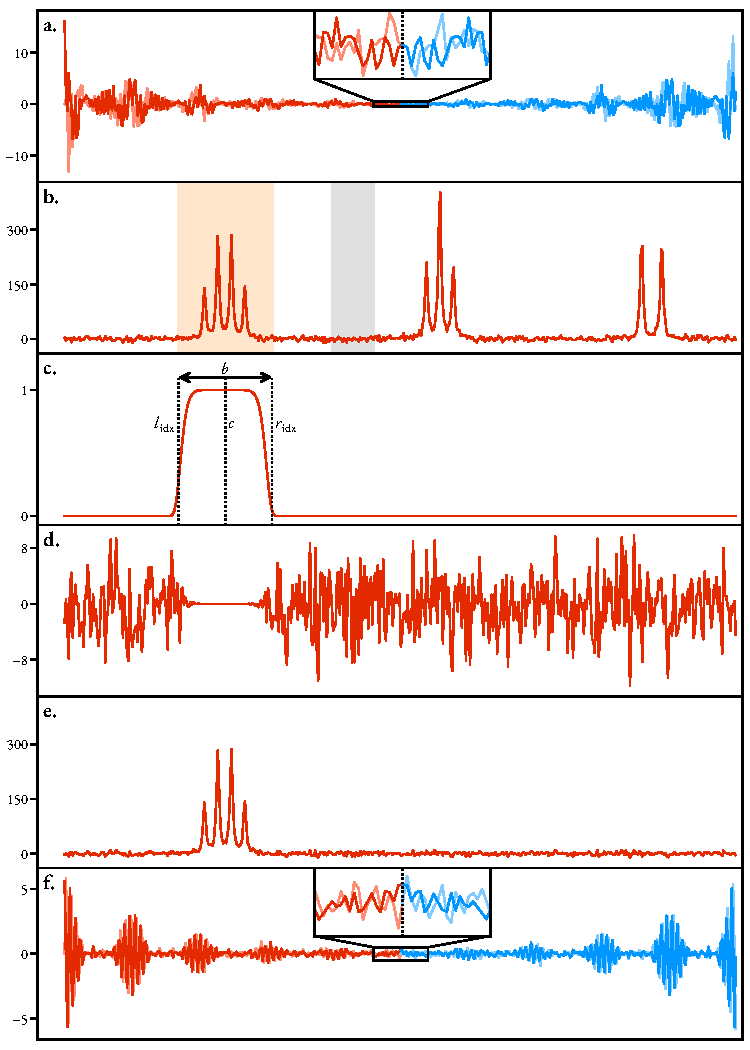
\includegraphics{filtering/filtering.pdf}
     \caption[
         An illustration of the filtering procedure applied to a \acs{1D}
         \acs{FID}.
     ]{
         An illustration of the filtering procedure applied to a \ac{1D}
         \ac{FID}.
         \textbf{a.} A \ac{VE} $\by_{\text{ve}}$, with the first and last
         $N$ points coloured red and blue, respectively. The middle of the
         \ac{VE} is magnified to highlight its conjugate symmetry.
         \textbf{b.} The \ac{FT} of the \ac{VE}, $\symbf{s}_{\text{ve}}$.
         The region of interest (orange) and noise region (grey) are denoted.
         \textbf{c.} A super-Gaussian function used as a band-pass filter,
         $\symbf{g}$.
         \textbf{d.} \acs{AWGN} vector to be added to the filtered spectrum.
         The magnitude of the signal at each point is dependent on the
         corresponding super-Gaussian value.
         \textbf{e.} The filtered spectrum $\widetilde{\symbf{s}}_{\text{ve}}$,
         formed by applying the super-Gaussian filter, and adding the noise
         vector.
         \textbf{f.} The \ac{IFT} of the filtered spectrum,
         $\widetilde{\symbf{y}}_{\text{ve}}$, from which the final filtered
         signal $\widetilde{\symbf{y}}$ is obtained by extracting
         the first $N$ points.
     }
     \label{fig:filtering}
\end{figure}

The central index and bandwidth of the super-Gaussian filter function are given
by the following expressions:
\begin{subequations}
    \begin{gather}
        c = \tfrac{1}{2} \left(l_{\text{idx}} + r_{\text{idx}}\right), \\
        b = l_{\text{idx}} - r_{\text{idx}},
    \end{gather}
\end{subequations}
where $l_{\text{idx}}$ and $r_{\text{idx}}$ denote the desired
indices where the filter's left and right bounds are located, respectively.
Array indices can be obtained from the corresponding spectral frequencies
$f^{(d)}_{\unit{\hertz}}$ via
\begin{equation}
    \begin{gathered}
        f_{\text{idx}} =
            \left \lfloor
                \frac
                {
                    \left(2N - 1\right)
                    \left(\fsw + 2 \left(\foff - f_{\unit{\hertz}}\right) \right)
                }
                {2 \fsw}
            \right \rceil \\
        \forall f_{\unit{\hertz}} \in
            \left[\foff - \tfrac{1}{2} \fsw, \foff + \tfrac{1}{2} \fsw\right].
        \label{eq:fidx}
    \end{gathered}
\end{equation}
Conversion from \unit{\partspermillion} to array indices can be achieved by
replacing  $f_{\unit{\hertz}}$ in \eqref{eq:fidx} with
$f_{\unit{\partspermillion}} f_{\text{sfo}}$, where $f_{\text{sfo}}$ is the
transmitter frequency (\unit{\mega \hertz}) and $f_{\unit{\partspermillion}}$
is the frequency expressed as a chemical shift.

\subsubsection{Spectrum slicing}
Thus far, the method described is able to reduce the model order of a given
signal, however the signal still comprises the same number of points. However
it is clear that there are a large number of points outside the region of
interest in $\widetilde{\symbf{s}}_{\text{ve}}$ that do not possess any
meaningful information. Discarding such points will then lead to filtered
\ac{FID} with the same information about the signals of interest, but with
far fewer points. A slicing ratio is defined, $\chi \in \mathbb{R}: \chi>
1$,
which dictates the left and right indices at which the spectrum should be
sliced:
\begin{subequations}
    \begin{gather}
        l_{\text{slice}} =
        \begin{cases}
            c - \left \lfloor \frac{b \chi}{2} \right \rfloor &
            \text{if } \geq 0 \\
            0 & \text{otherwise}
        \end{cases} \\
        r_{\text{slice}} =
        \begin{cases}
            c + \left \lceil \frac{b \chi}{2} \right \rceil &
            \text{if } \leq 2N - 1 \\
            2N - 1 & \text{otherwise}
        \end{cases}
    \end{gather}
\end{subequations}
The filtered spectrum is then sliced accordingly:
\begin{equation}
    \widetilde{\symbf{s}}_{\text{ve,slice}} =
        \widetilde{\symbf{s}}_{\text{ve}} [
            l_{\text{slice}} :
            r_{\text{slice}} + 1
        ].
\end{equation}
Generation of the final sub-\ac{FID} is then achieved in a similar fashion to
before: by performing \ac{IFT}, and retaining the first half of the signal.
It is also necessary to scale the signal by the ratio of the number of points
in the sliced spectrum and it's unsliced counterpart, in order to ensure that
the amplitudes of each signal are unaffected.
\begin{subequations}
    \begin{gather}
        \widetilde{\by} =
            \frac{r_{\text{slice}} - l_{\text{slice}}}{2N}
            \IFT(\widetilde{\symbf{s}}_{\text{ve,slice}})
            [0 : N_{\text{slice}}],\\
            N_{\text{slice}} = \left \lfloor \frac{r_{\text{slice}} - l_{\text{slice}}}{2} \right \rfloor
    \end{gather}
\end{subequations}
The associated sweep width and transmitter offset of the \ac{FID} will have
been altered by this process, and in order to derive accurate frequencies and
damping factors for the sliced signal, it is necessary to determine these. The
corrected values can be computed using
\begin{subequations}
    \begin{gather}
        f_{\text{sw,slice}} = \frac{r_{\text{slice}} - l_{\text{slice}}}{2N - 1} \fsw\\
        f_{\text{off,slice}} = \foff + \frac{\fsw}{2} \left(
            1 - \frac{l_{\text{slice}} + r_{\text{slice}}}{2N - 1}
        \right)
    \end{gather}
\end{subequations}
